\documentclass[xcolor=dvipsnames,12pt]{beamer}
\usecolortheme[named=RoyalPurple]{structure}
\useoutertheme{infolines}
\usetheme{CambridgeUS}
%\usetheme[height=14mm]{Rochester}
%\hypersetup{colorlinks=true,linkcolor=yellow}
\setbeamertemplate{items}[ball]
\setbeamertemplate{blocks}[rounded][shadow=true]
\setbeamertemplate{navigation symbols}{}
\usepackage{color}
%\usefonttheme{structuresmallcapsserif}
%\usefonttheme{professionalfonts}
%\useoutertheme{default}
%\useoutertheme{infolines}


%\documentclass{beamer}
%\usecolortheme{structure}
\usepackage{graphicx}
%\usetheme{PaloAlto}
%\setbeamertemplate{items}[ball]
%\setbeamertemplate{blocks}[rounded][shadow=true]
%\useoutertheme{umbcfootline}
\newtheorem{assume}{\rlap{A}\hskip .1in}
%\newtheorem{result}{Result}[chapter]
\newcommand{\Var}  {\mbox{Var}}
\newcommand{\V} {\mbox{V}}
\newcommand{\E}  {\mbox{E}}
\newcommand{\PR}  {\mbox{P}}
\newcommand{\diag} {\operatorname*{diag}}
\newcommand{\tr} {\mbox{tr}}
\newcommand{\bmw}[1]{{\mbox{$#1$}}}
\newcommand{\MSE}{\mbox{MSE}}
\newcommand{\MSPE}{\mbox{MSPE}}


\def\bmh{{\hat \mathbf m}}
\def\bm{{\mathbf m}}
\def\bn{{\mathbf n}}
\def\mh{{\hat m}}
\def\bOmega{{\mathbf \Omega}}
\def\be{{\mathbf e}}
\def\bs{{\mathbf s}}
\def\by{{\mathbf y}}
\def\b1{{\mathbf 1}}
\def\bx{{\mathbf x}}
\def\bw{{\mathbf w}}
\def\bzero{{\mathbf 0}}

\def\bP{{\mathbf P}}
\def\bI{{\mathbf I}}
\def\bM{{\mathbf M}}
\def\bH{{\mathbf H}}
\def\bN{{\mathbf N}}
\def\bW{{\mathbf W}}
\def\bX{{\mathbf X}}
\def\bZ{{\mathbf Z}}
\def\bT{{\mathbf T}}
\def\bV{{\mathbf V}}
\def\bC{{\mathbf C}}
\def\bG{{\mathbf G}}
\def\bY{{\mathbf Y}}
\def\bD{{\mathbf D}}
\def\bS{{\mathbf S}}
\def\bR{{\mathbf R}}

\def\bbeta{\mbox{\boldmath $\beta$}}
\def\bepsilon{\mbox{\boldmath $\varepsilon$}}

% items enclosed in square brackets are optional; explanation below
\title[]{Part 8}
%\subtitle[ttt]{}
\author[Stat 801]{Linear Regression\\
Intercept, Slope\\
Inference about the Intercept and Slope\\
F test and ANOVA\\
Prediction\\
Lack of Fit of the Linear Model\\
Correlation\\
Residual Analysis}
\date{}

\begin{document}

\begin{frame}[plain]
  \titlepage
\end{frame}




\begin{frame}
\frametitle{LINEAR REGRESSION  AND CORRELATION}
\begin{itemize}
\item Consider \textcolor{magenta}{\textit{bivariate data}} consisting of ordered pairs
of numerical values ($x,y$).  
\item Often such data arise by setting an
$x$ variable at certain fixed values (which we will call
\textcolor{magenta}{levels}) and taking a random sample from the population
of $Y$ that is assumed to exist at each of the levels of $x$.
\item Here we are thinking of $x$ as  \textcolor{magenta}{not being  a random variable}, 
because we are considering only selected fixed values of $x$ (for 
sampling purposes).
\item However, $Y$ is a random variable and we define 
 $Y$ on the population that exists at each level of $x$.
 \end{itemize}
\end{frame}

\begin{frame}
\begin{itemize}
\item Graphically, a scatterplot of the data  depicting the $y$-values
obtained by sampling the  populations at each of the pre-selected $x$-values might appear as follows:
\end{itemize}
\begin{picture}(130,120)(-30,-30)
\put(5,5){\vector(1,0){70}}
\put(5,5){\vector(0,1){70}}
\put(10,4){\line(0,1){2}}
\put(10,-5){\circle*{1}}
\put(10,-10){\circle*{1}}
\put(10,8){\circle*{1}}
\put(10,15){\circle*{1}}
\put(20,4){\line(0,1){2}}
\put(20,-8){\circle*{1}}
\put(20,-20){\circle*{1}}
\put(20,15){\circle*{1}}
\put(20,35){\circle*{1}}
\put(20,45){\circle*{1}}
\put(25,4){\line(0,1){2}}
\put(25,25){\circle*{1}}
\put(25,30){\circle*{1}}
\put(25,40){\circle*{1}}
\put(25,55){\circle*{1}}
\put(35,4){\line(0,1){2}}
\put(35,10){\circle*{1}}
\put(35,20){\circle*{1}}
\put(35,28){\circle*{1}}
\put(35,42){\circle*{1}}
\put(35,50){\circle*{1}}
\put(55,4){\line(0,1){2}}
\put(55,18){\circle*{1}}
\put(55,23){\circle*{1}}
\put(55,27){\circle*{1}}
\put(55,33){\circle*{1}}
\put(55,47){\circle*{1}}
\put(68,-2){x}
\put(-2,70){y}
\end{picture}
\end{frame}


\begin{frame}
Our objectives given such data are usually twofold:
\begin{itemize}
\item \textcolor{magenta}{Summarize} the characteristics of the $Y$ populations
      across values of $x$ --  \textcolor{magenta}{Fit the Model}
\item  \textcolor{magenta}{Interpolate} between levels of $X$ to estimate
      parameters of $Y$ populations from which samples were
      not taken --  \textcolor{magenta}{Prediction}
\item The center of our attention is usually on the  \textcolor{magenta}{means} of the
$Y$ populations, $E(Y)$, and especially their  \textcolor{magenta}{relationship to one another}.\\[.1in]
\item Considering various relationships among these population means is called \textcolor{magenta}{parametric modeling}.
\end{itemize}
\end{frame}


\begin{frame}
\begin{itemize}
\item  {\textcolor{magenta}{\textit{The simple linear regression model}}} says that the 
populations at each $x$-value are normally distributed
and that the means of these normal distributions all fall on a straight line, called the \textcolor{magenta}{\textit{regression line.}}\\[.1in]
\begin{center}
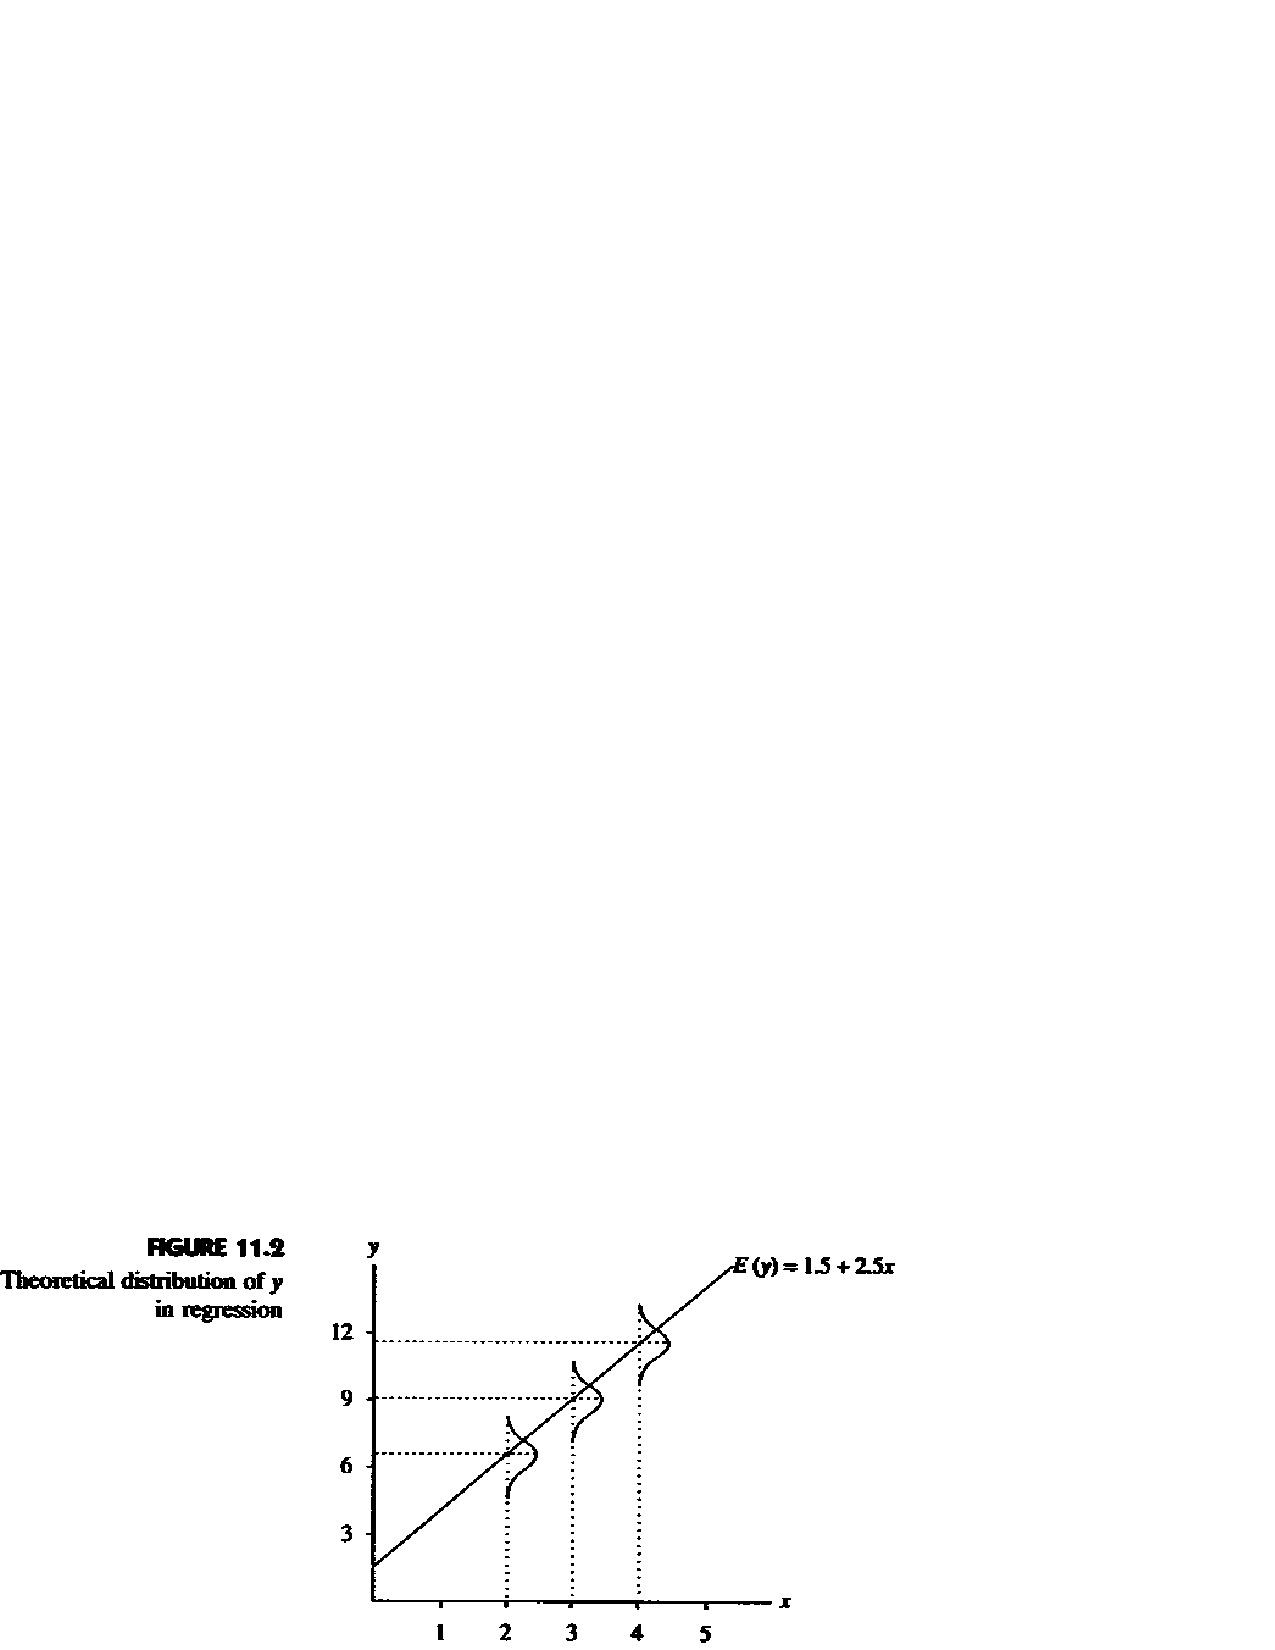
\includegraphics[trim=0 0 10 500,clip,scale=0.5]{fig11_2.pdf}\\[.1in]
\end{center}
%\vspace*{-.3in}
\end{itemize}
\end{frame}




\begin{frame}
\begin{itemize}
\item Let us begin by considering a \textcolor{magenta}{linear relationship} among
population means.\\[.01in] 
\item The equation of a straight line through
means $E(Y)$ across $x$-values can be written as
$E(Y) = \beta_0 + \beta_1x$\\[.01in]
\item Here $\beta_0$ is the \textcolor{magenta}{\textit{intercept}} and $\beta_1$ is the
\textcolor{magenta}{\textit{slope}} of the line.\\[.01in]
%**********************************************************
\begin{picture}(120,80)(-35,0)
\setlength{\unitlength}{.5mm}
\put(5,5){\vector(4,0){60}}
\put(5,5){\vector(0,4){50}}
\put(58,-2){$x$}
\put(-15,48){E(Y)}
\put(-5,15){\line(5,2){65}}
\put(-2,20){\small{$\beta_0$}}
\put(22,26){\line(1,0){20}}
\put(42,26){\line(0,1){8}}
\put(43,29){\small{$\beta_1$}}
\put(33,21){\small{$1$}}
\end{picture}
\end{itemize}
\end{frame}



\begin{frame}
\begin{itemize}
\item The $y$-values observed at each  $x$-value  is assumed to be 
a random sample from a \textcolor{magenta}{normal distribution} with the \textcolor{magenta}{mean} 
$E(Y)=\beta_0 + \beta_1x$, i.e., the mean is a linear function of
$x$.
\item  The \textcolor{magenta}{variance} of the normal distributions
at each  $x$-value is assumed to be the same (or constant).
\item Thus the
$y$-values can be related to the $x$-values through the
relationship
\begin{equation}
y = \beta_0 + \beta_1\,x + \epsilon  
\end{equation}  
\item Here $\epsilon$ is a random variable (called \textcolor{magenta}{random error})
with mean zero i.e, $(E(\epsilon)=0)$, and variance $\sigma_{\epsilon}^2$.
\item This model says that sample values are 
random distances from the line $\mu = \beta_0 + \beta_1\,x$ at each 
 $x$-value. 
\end{itemize}
\end{frame}


\begin{frame}
\begin{itemize}
\item The unknown constants in Equation (1), $\beta_0$, $\beta_1$, and   $\sigma_{\epsilon}^2$ are called the \textcolor{magenta}{\textit{parameters}} of the model.\\[.01in]
\item The next question we consider is ``How do we proceed to derive
a \textcolor{magenta}{\textit{good}} approximating line through $Y$ population means,
given only samples from some of the $Y$ populations?''\\[.01in]
\item  In other
words, we need to obtain \textcolor{magenta}{\textit{good}} estimates of the parameters 
of the model  using the  observed data.\\[.01in]
\item The phrase \textcolor{magenta}{\textit{fitting a line through the
data}} is used to describe our problem.\\[.01in]
\item It is easy to imagine simply \textcolor{magenta}{\textit{eye-balling}} a line through
the points on the scatterplot. But is  hard to imagine in what way this can be considered a \textcolor{magenta}{\textit{good}} line. 
\end{itemize}
\end{frame}




\begin{frame}
\begin{itemize}
\item The  \textcolor{magenta}{\textit{method of least squares}} provides
a more sound and clearly defined procedure for fitting a line.\\[.01in]  
\item As an example, consider
the data in Section 11.2:\\[.1in]
 \textcolor{red}{Example: Road Surfacing Data}\\[-.2in]
\begin{center}
\begin{tabular}{l|rrrrr}\hline
Project & 1 & 2 & 3 & 4 & 5 \\ \hline
Cost $y_i$(in \$1000's) & 6.0 & 14.0 & 10.0 & 14.0 & 26.0  \\
Mileage (in miles) & 1.0 & 3.0 & 4.0 & 5.0 & 7.0 \\\hline \\[.01in]
\end{tabular}
\end{center}
\item In this example, as well as in other examples in this Chapter,
for simplicity we will assume that ony one
$y$-value has been observed at each of the $x$-values.
\end{itemize}
\end{frame}



\begin{frame}
\begin{itemize}
\item To explain this method we must first define the terms
 \textcolor{magenta}{\textit{predicted value}} and  \textcolor{magenta}{\textit{residual}}.\\[.1in]
\item The method of least squares selects a specific line which is
claimed to be good.  It does so by estimating a
value $\hat{\beta}_0$ for $\beta_0$ and $\hat{\beta}_1$
for $\beta_1$ using the observed data.\\[.1in] 
\item  \textcolor{magenta}{The least squares} line then has equation
$$
  \hat{y} = \hat{\beta}_0 + \hat{\beta}_1\,x
$$
where $\hat{y}$ is the point estimate of the mean of the
population that exists at $x$. 

\end{itemize}
\end{frame}


\begin{frame}
\begin{itemize}
\item The \textcolor{magenta}{predicted value} $\hat{y}_i$ at a particular value of $x_i$, 
 is the value of  $y$ predicted
by the model at that value of $x_i$ i.e., $\hat{y}_i=\hat{\beta}_0+\hat{\beta}_1 x_i$\\[.1in] 
\item The \textcolor{magenta}{residual} is the difference between an observed value $y$
at a given value of $x_i$, and  $\hat{y}_i$ i.e., $(y_i - \hat{y}_i).$\\[.1in]
\begin{center}
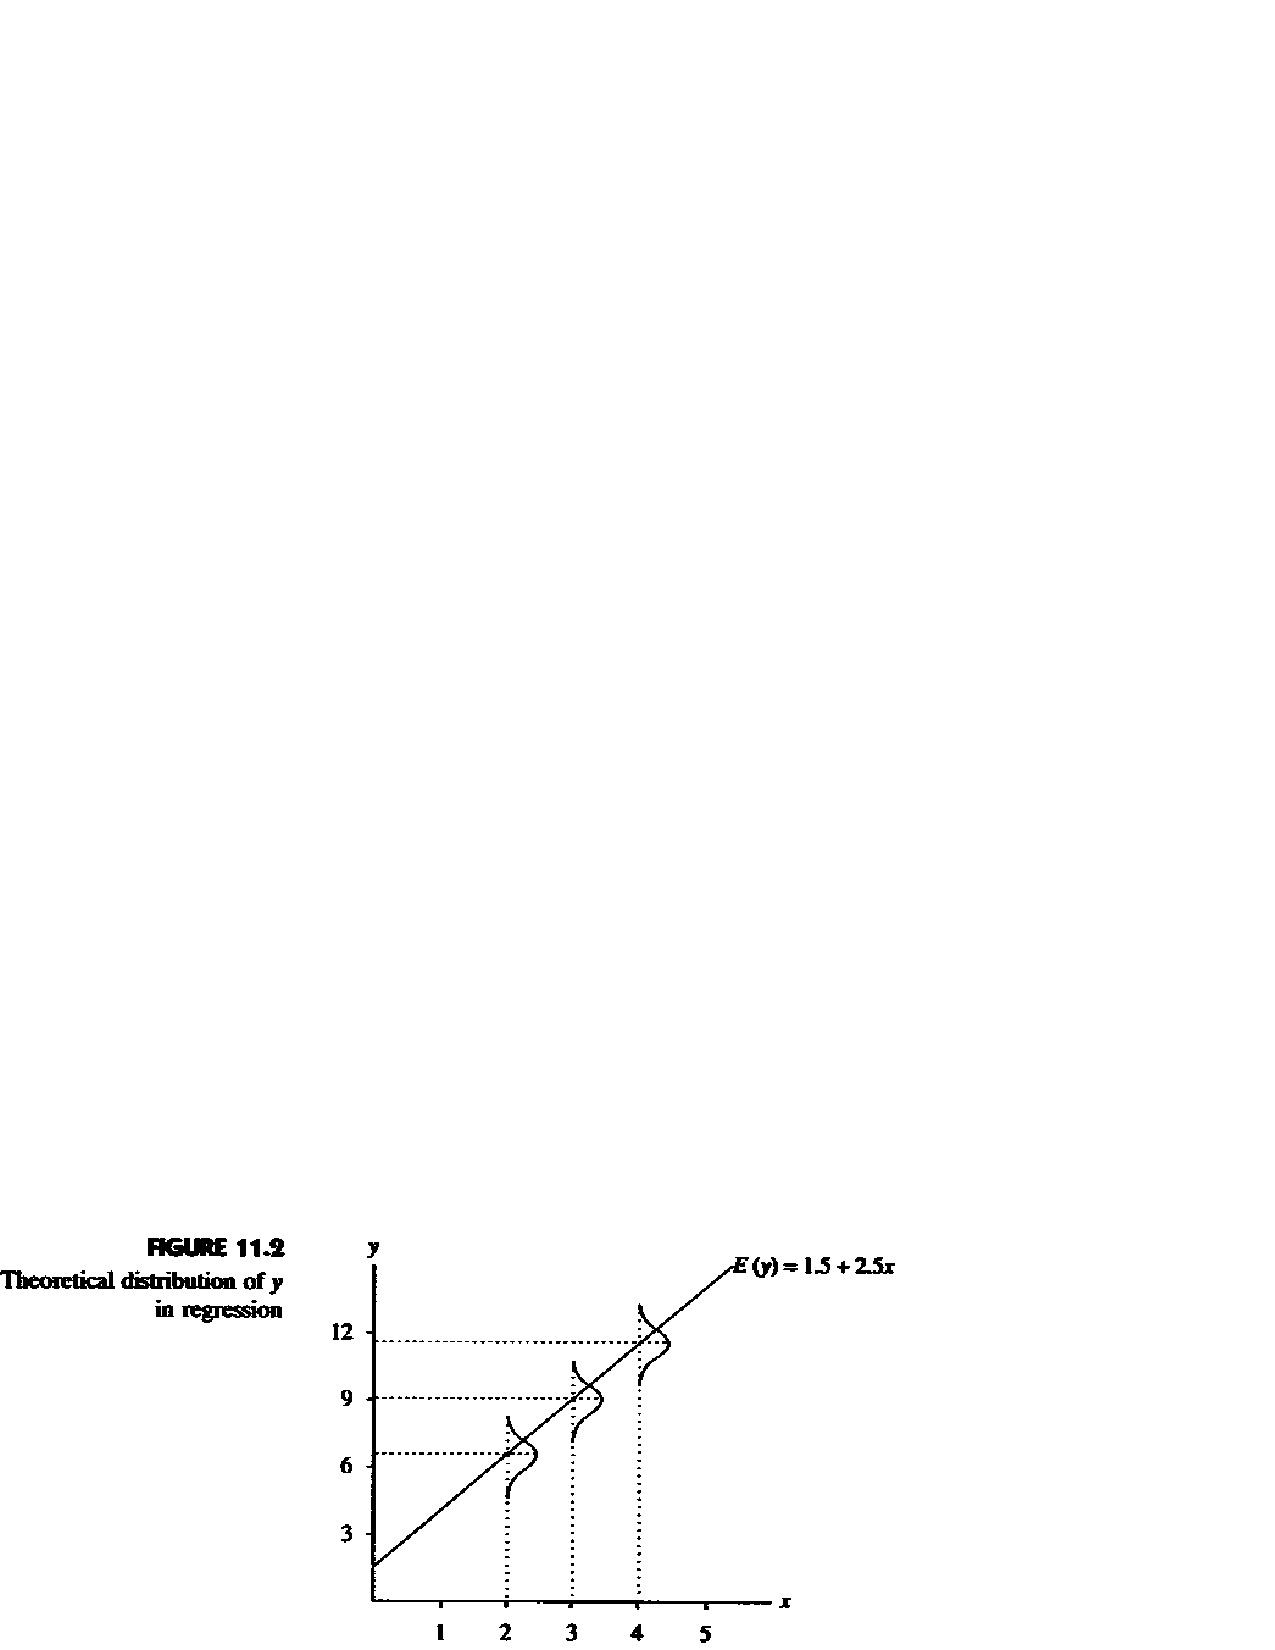
\includegraphics[trim=0 0 10 500,clip,scale=0.5]{fig11_2.pdf}\\[.1in]
\end{center}
\end{itemize}
\end{frame}


\begin{frame}
\begin{itemize}
\item The residual $y-\hat{y}$ is the ``estimate'' $\hat{\epsilon}$ 
of $\epsilon$, i.e., it is a prediction of the sampling error in $y$ under the
assumption that the population means lie on a straight line.\\[.1in]
\item The method of least squares selects that line 
which produces the smallest value of the sum of
squares of all residuals (hence the name  \textcolor{magenta}{least squares}).\\[.1in]
\item That is, the estimates $\hat{\beta}_0$ and $\hat{\beta}_1$ are chosen to
minimize
$$
 \sum_i \, (y_{i} - \hat{y}_{i})^2 = \sum_i \, (y_{i} - \hat{\beta}_0 - \hat{\beta}_1 \,x_i)^2
$$
 where $(x_i,\, y_i) \ \ i=1,2,\ldots,n$ are pairs of observations.
\end{itemize}
\end{frame}



\begin{frame}
\begin{itemize}
\item Thus $\hat{\beta}_0$ and $\hat{\beta}_1$ are called the   \textcolor{magenta}{least
squares estimates}  (L.S. estimates ) of $\beta_0$ and 
$\beta_1$, respectively.\\[.1in]
\item The  L.S. estimates $\hat{\beta}_0$ and $\hat{\beta}_1$
given data pairs ($x,y$) are calculated using the formulae:
\begin{eqnarray*}
  \hat{\beta}_1 &=& S_{xy}/S_{xx} \qquad \qquad \hat{\beta}_0 = \bar{y} -
                             \hat{\beta}_1 \bar{x} \\[.1in]
\mbox{where}  \ \ \   S_{xx} & = & \sum(x-\bar{x})^2\\
    S_{xy} &=& \sum(x-\bar{x})(y-\bar{y})
\end{eqnarray*}
\end{itemize}
\end{frame}


\begin{frame}
Handout Example 11.2
\end{frame}



\begin{frame}
After we obtain a least squares fitted line, we are then usually
interested in seeing how well the line appears to go through $Y$
population means.  One way to investigate this is to look at
relative magnitudes of certain sums of squares.  
\begin{itemize}
\item The  \textcolor{magenta}{Total Variation} in all the sample $y$ values is
measured by the quantity $\frac{1}{n-1} \sum_{i=1}^n (y_{i} - \bar{y})^2 $
\item Let us consider only  the numerator\\[.1in]
 $\mbox{\textcolor{magenta}{Total~Sum~of~Squares}} = \mbox{SSTot}= \sum_{i=1}^n (y_{i} -  \bar{y})^2$\\[.1in]
 \end{itemize}
A little algebraic manipulation will result in the following partitioning of the total sum of squares:\\[.1in]
 $\sum_{i=1}^n\, (y_{i} - \bar{y})^2 =\sum_{i=1}^n \, (y_{i} - \hat{y}_i)^2 +\sum_{i=1}^n  \hat{y}_i - \bar{y})^2$
\end{frame}



\begin{frame}
\begin{itemize}
\item  We interpret this by noting that the measure of total variation,
which is the left part of the equation, is expressible as the
sum of two parts which constitute the right side. \\[.01in] 
\item The first
part of the right side is the sum of squared residuals  \\[.05in] 
$\mbox{\textcolor{magenta}{Residual~Sum~of~Squares}} = \mbox{SSE} = \sum_{i=1}^n \, (y_{i} - \hat{y}_i)^2$.\\[.01in]
\item We would expect residuals to be  close to zero if
the $Y$ population means lie close to the estimated
least squares line. Thus the smaller the value of SSE
closer the regression line will be to the data.\\[.05in]
\item The other term in the right side of the algebraic identity is \\[.05in]
  $ \mbox{\textcolor{magenta}{Regression~Sum~of~Squares}}= \mbox{SSReg} =  \sum_{i=1}^n \, (\hat{y}_i - \bar{y})^2$
\end{itemize}
\end{frame}




\begin{frame}
\begin{itemize}
\item Since the left side is the sum of two positive quantities, when SSE decreases SSReg must increase and vice versa.\\[.1in]
\item The identity is the basis for \textcolor{magenta}{analysis of variance for
regression} summarized below: \\[-.3in]
\begin{center}
\begin{normalsize}
\begin{tabular}{l@{\extracolsep{.5in}}ccl} \hline
Source& df & Sum of  & Mean  \\
     &   & Squares & Square  \\ \hline
Reg & 1 & SSReg &  \rm{MSReg}=SSReg/1  \\[.1in]
Error & n-2  & SSE & MSE=SSE/(n-2)  \\[.1in] 
Total & n-1 & SSTot \\ \hline
\end{tabular}
\end{normalsize}
\end{center}
\item Later we shall add another column to the above table for calculating an F-statistic 
for testing a hypothesis about $\beta_1$ 
\end{itemize}
\end{frame}




\begin{frame}
\frametitle{Interpretation of the Slope Parameter}
\begin{itemize}
\item In any straight line equation $y=a +bx$, the slope $b$ measures 
the change in the $y$-value for a unit change in the $x$-value
(rate of change in  $y$).
\item If $b$ is positive  $y$ would increase as  $x$ increases and if
$b$ is negative $y$ would decrease as  $x$ increases.
\item In the fitted regression model $  \hat{y} = \hat{\beta}_0 +
\hat{\beta}_1\,x$, the slope $\hat{\beta}_1$ is the change
$y$-value for  a unit change in the $x$-value predicted by the
fitted model.
\end{itemize}
\end{frame}



\begin{frame}
\begin{itemize}
\item As in the case when we estimated $\mu$ in a single sample case
or  $\mu_1-\mu_2$ in the 2 sample case, we need to obtain the
standard error of the estimate of $\hat{\beta_1}$ (and of  
$\hat{\beta_0}$). 
\item These indicate how accurate our estimates are
and help construct confidence intervals and perform tests of
hypotheses about the true parameter values $\beta_0$ and  $\beta_1$.
\end{itemize}
\end{frame}



\begin{frame}
\begin{itemize}
\item The standard deviation of $\hat{\beta_1}$, the slope parameter
is given by 
$$ \sigma_{\hat{\beta_1}}=\frac{\sigma_{\epsilon}}{\sqrt{S_{xx}}}$$
\item If the error variance $\sigma_{\epsilon}$ is large, then
$\sigma_{\hat{\beta_1}}$ would be large. 
\item This says that the slope 
parameter is estimated with high variability. 
\item That is, our estimate
of the rate of change in $y$ will be less accurate, which will
result in, say, a wider confidence interval for $\hat{\beta_1}$.
\end{itemize}
\end{frame}


\begin{frame}
\begin{itemize}
\item By the above formula, we see that the  standard deviation of 
$\hat{\beta_1}$ is also affected by $S_{xx}$.
\item That is smaller  $S_{xx}$ the
larger $\sigma_{\hat{\beta_1}}$ would be.  
\item $S_{xx}$ measures the spread of the $x$-values around its mean. If all the $x$-values crowd around the mean $\bar{x}$, then  $S_{xx}$ will be small.
\item In regression this does not help to estimate parameters of the 
model because the responses to other possible $x$-values will not be available.
\item If we have not selected enough $x$-values to cover the range of possible
$y$-values we want to predict, then the model we built will not be
able to predict changes in those $y$'s with enough accuracy. 
\end{itemize}
\end{frame}


\begin{frame}
\begin{itemize}
\item To estimate the above standard deviation we need an estimate
of $\sigma_{\epsilon}$. 
\item Since $\sigma_{\epsilon}^2$ is the variance
of the random errors $\epsilon_1,\,\epsilon_2,\ldots,\epsilon_n$,
we would construct estimate of  $\sigma_{\epsilon}^2$ based on 
the residuals $\hat{\epsilon_i}=y_i - \hat{y}_i,\ 
i=1,2,\ldots,n$. 
\item The estimator of $\sigma_{\epsilon}^2$ is 
$$s_{\epsilon}^2=\frac{ \sum_i (y_i -
\hat{y}_i)^2}{n-2}=\frac{\mbox{SSE}}{n-2}=MSE$$
\end{itemize}
\end{frame}


\begin{frame}
\begin{itemize}
\item Recall that for the sample variance $s^2$ of a sample 
$y_1, y_2, \ldots, y_n$, we divide $ \sum_i (y_i -\bar{y})^2$ 
by $n-1$ because with $\bar{y}$ we were estimating a single 
parameter $\mu$. 
\item In the estimate  $ s_{\epsilon}^2$
for the sample variance of the residuals, the  divisor 
is $n-2$ because in $\hat{y}= \hat{\beta}_0 + \hat{\beta}_1\,x$ we
are estimating 2 parameters: $\beta_0$ and  $\beta_1$. 
\item We say that
the Residual~SS has $n-2$ degrees of freedom.
 Using the estimate $s_{\epsilon}$ of $\sigma_{\epsilon}$ as
defined above, the standard error of  $\hat{\beta}_1$ is
$$ s_{\hat{\beta_1}}=\frac{s_{\epsilon}}{\sqrt{S_{xx}}}$$
\end{itemize}
\end{frame}



\begin{frame}
\begin{itemize}
\item The standard error of $\hat{\beta_0}$, the intercept parameter
is similarly given by 
$$ s_{\hat{\beta_0}}= s_{\epsilon}\sqrt{\frac1n + \frac{\bar{x}^2}{S_{xx}}}$$
\item Thus The standard error of $\hat{\beta_0}$ is also affected by the choice of the $x$'s.
\item  The intercept estimate is the predicted value of $y$ at $x=0$.
\item In many experimental situations the estimate of the intercept is not of interest as 
as a value of zero for $x$ is not possible. 
\item \textbf{\textcolor{magenta}{Refer to the Analysis of Example 11.2: Pharmacy Data}}
\end{itemize}
\end{frame}



\begin{frame}
\frametitle{Computations in the Simple Linear Regression Model}
 In the textbook, for Example 11.2, the quantities $S_{xx},\,S_{xy}$ were computed
by first computing the sum of the deviations $(x-\bar{x}),\, (y-\bar{y})$ and the sum of the products $(x-\bar{x})(y-\bar{y})$.\\
 In practice,
however, the following formulas can be used in hand computations. 
Thus the computation of the deviations is not necessary:
$$S_{xx} = \sum x^2 - \frac{(\sum x)^2}{n}$$\\
$$S_{xy} = \sum xy - \frac{(\sum x)(\sum y)}{n}$$\\
$$S_{yy} = \sum y^2 - \frac{(\sum y)^2}{n}$$
\end{frame}




\begin{frame}
 In Example 11.2, the quantities needed are
 \begin{itemize}
\item  $ \sum x = 338,\quad \sum y =713 ,\quad \sum x^2=14,832\, , $
\item $\sum xy=30,814,\quad \sum y^2=64,719, \quad n=10$
\item $S_{xx} = \sum x^2 - \frac{(\sum x)^2}{n}=14,832-\frac{338^2}{10}=3,407.6$
\item $S_{xy} = \sum xy - \frac{(\sum x)(\sum y)}{n}
            =30,814-\frac{(338)(713)}{10}=6,714.6$
\item $S_{yy} = \sum y^2 - \frac{(\sum y)^2}{n}=64,719-\frac{713^2}{10}=13,882.1$
\end{itemize}
\end{frame}




\begin{frame}
These could be used to obtain the estimates $\hat{\beta_0}$ and
$\hat{\beta_1}$ as before:
\begin{itemize}
\item $\hat{\beta_1} = S_{xy}/S_{xx} =6,714.6/3,407.6=1.97048$
\item $\hat{\beta_0} = \bar{y}-\hat{\beta_1} \bar{x}=71.3-(1.97048)(33.8)=4.6979$
\end{itemize}
In addition, the following formulas are
needed to compute the quantities for an  \textcolor{magenta}{analysis of variance}
or \textcolor{magenta}{ANOVA} table:
\begin{itemize}
\item ${SSTot} =  S_{yy}=13,882.1$
\item ${SSReg} =\frac{S_{xy}^2}{S_{xx}}=13,230.97 $
\item ${SSE  } = S_{yy}-\frac{S_{xy}^2}{S_{xx}}=13,882.1-13,230.97=651.13$
\end{itemize}
\end{frame}




\begin{frame}
This gives the following \textcolor{magenta}{ANOVA table}:
\begin{center}
\begin{tabular}{l@{\extracolsep{.5in}}crr} \hline
Source& df & Sum of  & Mean  \\
     &   & Squares & Square  \\ \hline 
Regression & 1 &   13,230.97 & 13,230.97  \\
Error & 8 & 651.13 & 81.39  \\
Total & 9 & 13,882.1 \\ \hline\\
\end{tabular}
\end{center}
\end{frame}



\begin{frame}
\frametitle{Coefficient of Determination:}
$$
  r^2 = \frac{\sum(\hat{y}-\bar{y})^2}{\sum(y-\bar{y})^2}
=\frac{\mbox{SSReg}} {\mbox{SSTot}}=\frac{ 13,230.97}{
13,882.1}=.9531\approx 95\% 
$$
This is a measure of how much better the regression model 
does in predicting $y$ than just using $\bar{y}$ to 
predict  $y$.
\end{frame}





\begin{frame}
\frametitle{Inferences about {\boldmath$\beta_0$} and {\boldmath$\beta_1$}}
 We are still considering the model
$$
  y = \beta_0 + \beta_1x + \epsilon, 
$$
and the least squares fit using a random sample ($x_i, y_i$),
$i=1,2, \ldots n$
$$
  \hat{y} = \hat{\beta}_0 + \hat{\beta}_1 x
$$
is the prediction equation, and the L.S. estimates have form
$$
  \hat{\beta}_1 = S_{xy}/S_{xx} \qquad \hat{\beta}_0 = \bar{y} -
  \hat{\beta}_1 \bar{x} \ .
$$
\end{frame}


\begin{frame}
\begin{itemize}
\item We have assumed that the $Y$ population at each value of $x$ is
Normal with mean $\beta_0 + \beta_1x$\\[.1in]
\item Each population has the same variance
$\sigma_\epsilon^2$ \\[.1in]
\item Under these assumptions, the least squares estimators
$\hat{\beta}_0$
and $\hat{\beta}_1$ are each normally distributed:
\begin{eqnarray*}
  \hat{\beta}_1 &\sim& N\left(\beta_1,\sigma_{\hat{\beta_1}}^2\right)\\[.1in]
  \hat{\beta}_0 &\sim& N\left(\beta_0,\sigma_{\hat{\beta_0}}^2 \right)
\end{eqnarray*}
\end{itemize}
\end{frame}



\begin{frame}
\begin{itemize}
\item We have earlier shown that  the estimator of the standard
deviation of $\hat{\beta}_1$ is
$$ \hat{\sigma}_{\hat{\beta_1}}=s_{\hat{\beta_1}}=\frac{s_{\epsilon}}{\sqrt{S_{xx}}}$$
\item and that the estimator of the standard
deviation of  $\hat{\beta}_0$ is
$$\hat{\sigma}_{\hat{\beta_0}}= s_{\hat{\beta_0}}= s_{\epsilon}\sqrt{\frac1n + \frac{\bar{x}^2}{S_{xx}}},$$
\item In these formulas, $s_{\epsilon}=\sqrt{MSE}$\\[.15in]
\item Using the above results, confidence intervals and tests
about the parameters $\beta_1$ (and $\beta_0$) can be obtained.
\end{itemize}
\end{frame}


\begin{frame}
\textbf{\textcolor{blue}{ A {\boldmath$100(1-\alpha)$}\% Confidence Interval for {\boldmath$\beta_1$}:}}\\[.1in]
$$
\hat{\beta}_1 \pm t_{\alpha/2}\,\cdot 
s_{\hat{\beta}_{1}} \quad  
\mbox{giving} \quad 
\hat{\beta}_1 \pm t_{\alpha/2}\,\cdot \frac{s_{\epsilon}}{\sqrt{S_{xx}}}
$$
 where $t_{\alpha/2}$ is the $100(1-\alpha/2)$ percentile 
of the student's $t$ distribution with $(n-2)$ degrees of freedom.\\[.15in]
\end{frame}



\begin{frame}
\textbf{\textcolor{blue}{Tests of Hypotheses About {$\beta_1$} }}\\[.1in]
\textbf{\textcolor{magenta}{Test:}}\\[-.7in]
\begin{tabbing}
xxxxxxx\= xxxx \= xxxxxx \= xxxxxxxxxxx \= xxxx \= xxxxxx \= \kill
\>$H_0:$ \> 1. $\beta_1 \leq 0$ \> \> $H_a:$ \> 1. $\beta_1 > 0$\\
\>$H_0:$ \> 2. $\beta_1 \geq 0$ \>\> $H_a:$ \> 2. $\beta_1 < 0$\\
\>$H_0:$ \> 3. $\beta_1 = 0$ \>\>   $H_a:$ \> 3. $\beta_1 \neq 0$\\
\end{tabbing}
\begin{tabbing}
xxxx \= xxxxxx \= xxxxxxxxxxx \= xxxx \= xxxxxx \= \kill
\textbf{\textcolor{magenta}{Test Statistic:}}  \>  \> \>$ t = \frac{\hat{\beta}_1-0}{s_\epsilon/\sqrt{S_{xx}}}$\\[.1in]
\textbf{\textcolor{magenta}{Rejection Region:}}  for specified $\alpha$ and $df= n-1$,\\[.1in]
\> \>  $\begin{array}{ll}
1. \ \mathrm{Reject~} H_0 \mathrm{~if~} t > t_{\alpha,\,(n-2)} & \\
2. \ \mathrm{Reject~} H_0 \mathrm{~if~} t < -t_{\alpha,\,(n-2)} & \\
3. \ \mathrm{Reject~} H_0 \mathrm{~if~} |t| >  t_{\alpha/2,\,(n-2)} &
\end{array}$ \\[-.5in]
\end{tabbing}
\end{frame}
\begin{frame}
 where $t_{\alpha,\,(n-2)}$ is the $100(1-\alpha)$ percentile of the student's
$t$ distribution with $(n-2)$ degrees of freedom.\\[.2in]
For a hypothesis like $H_0: \beta_1 = 3$, the test statistic is
modified as,
$$
  t = \frac{\hat{\beta}_1 - 3}{s_\epsilon/\sqrt{S_{xx}}}
$$
\end{frame}





\begin{frame}
\frametitle{An F-test from the analysis of variance table}
An alternative test of\\[.1in]
$H_0: \beta_1 = 0 \quad \mathrm{vs.} \quad H_a: \beta_1 \neq 0$\\[.1in]
which is more important in the  multiple regression case than our
simple linear regression models, comes from the 
\textcolor{magenta}{analysis of  variance table} given below.
\begin{center}
%\begin{normalsize}
\begin{tabular}{l@{\extracolsep{.2in}}llll} \hline
Source& df & Sum of  & Mean &F \\
     &   & Squares & Square  \\ \hline
Regression & 1 & SSReg &  MSReg & F=MSReg/MSE  \\[.1in]
Error & n-2  & SSE & MSE   \\[.1in] 
Total & n-1 & SSTot \\ \hline
\end{tabular}
%\end{normalsize}
\end{center}
\vspace*{.1in}
 The F test statistic computed above is used
for an $F$-distribution-based test with $df_1 = 1$ and  $df_2 = n-2$.
\end{frame}



\begin{frame}
Intuitively, large values of this ratio do indicate that the slope
$\beta_1$ is not zero.
\begin{tabbing}
xxxxxxxxxxxx \= xxxxxx \= xxxxxxx \= xxxx \= xxxxxx \= \kill
 \textbf{\textcolor{magenta}{Test:}}
$H_0:$  \>  $\beta_1 = 0$ \> \mbox{against}\> $H_a:$ $\beta_1 \neq 0$\\[.1in]
\textbf{\textcolor{magenta}{Test Statistic:}}  \>  \> $F = \frac{\mathrm{MSReg}}{\mathrm{MSE}}$\\[.1in]
\textbf{\textcolor{magenta}{Rejection Region:}} \> \> $\mathrm{Reject~} H_0 \mathrm{~if~} F > F_\alpha$  
\end{tabbing}
 where $F_\alpha$ is the $100(1-\alpha)$ percentile of the 
$F$ distribution with $df_1 = 1$ and  $df_2 = n-2$
\end{frame}



\begin{frame}
\frametitle{Example 11.6}
A simple linear regression model was fitted to the mean age, 
$x$, of executives of 15 firms in the food industry and the
previous year's percentage increase in earning per share of the
firms, $y$.\\
\begin{tiny}
\begin{tabular}[t]{lrrrrrrrrrr}
\hline 
Mean Age &38.2 &40.0 &42.5 &43.4 &44.6 &44.9 &45.0 &45.4 \\
\% Change(in earnings per share) &8.9 &13.0 &4.7 &-2.4 &12.5 &18.4
&6.6 &13.5  \\[.1in]
Mean Age &46.0 &47.3 &47.3 &48.0  &49.1  &50.5  &51.6\\
\% Change(in earnings per share)  &8.5  &15.3  &18.9  &6.0  &10.4
&15.9  &17.1\\ \hline \\[.1in]
\end{tabular}
\end{tiny}\\
\begin{itemize}
\item The quantities needed for the computation are \\
  $ \sum x = 683.8,\quad \sum y =167.3 ,\quad \sum x^2=31,358.58$\\
$ \sum xy=7,741.74,\quad \sum y^2=2,349.61$
\end{itemize}
\end{frame}



\begin{frame}
\begin{itemize}
\item Using these it follows that\\
$S_{xx} = \sum x^2 - \frac{(\sum x)^2}{n}
              =31,358.58-\frac{ 683.8^2}{15}=186.4173$\\
$S_{xy} = \sum xy - \frac{(\sum x)(\sum y)}{n}
            =7,741.74-\frac{(683.8)(167.3)}{15}$\\
$= 115.0907$\\
$S_{yy} = \sum y^2 - \frac{(\sum y)^2}{n}=2,349.61-\frac{167.3^2}{15}=
483.6573$
\item These could be used to obtain the estimates $\hat{\beta_0}$, 
$\hat{\beta_1}$, and $s_\epsilon=\sqrt{MSE}$ as before.
\end{itemize}
\end{frame}

\begin{frame}
\begin{itemize}
\item The calculations are:\\
$\hat{\beta_1} =S_{xy}/S_{xx} = 115.0907/186.4173=0.617382$\\
$\hat{\beta_0} = \bar{y}-\hat{\beta_1}
                    \bar{x}=11.153-(0.617382)(45.5867)=-16.991$\\
$SSE  = S_{yy}-\frac{S_{xy}^2}{S_{xx}}=483.6573-\frac{
115.0907^2}{186.4173}=412.60236$\\
$MSE   = SSE  /(n-2)=412.60236/13=31.7386$\\
$s_\epsilon=\sqrt{MSE}=5.634$
\item A $95\%$ confidence interval for $\beta_1$ is: \quad
$\hat{\beta}_1 \pm t_{.025,13}\,\cdot \frac{s_{\epsilon}}{\sqrt{S_{xx}}}$\\
\end{itemize}
\end{frame}


\begin{frame}
\begin{itemize}
\item It is calculated as:
$$
0.617382 \pm (2.16)(\frac{5.634}{\sqrt{186.4173}})\quad \mbox{or} \quad 
0.617382 \pm 0.89130
$$
i.e., $(-0.27392,\,1.5087)$.\\[.1in]
%\newpage
\item In this problem, to determine if executive age has any predictive
value for predicting change in earnings, we need to test 
\hspace{2in} $ H_0:\ \beta_1=0 \quad \mbox{vs.} \quad  H_a:\ \beta_1 \neq 0$\\[.1in]
\item We chose the two-sided research hypothesis because, if executive age
was a good predictor, we do not know whether it would have a
negative or a positive effect on  change in earnings. We use 
$\alpha=.05$ for the test.
\end{itemize}
\end{frame}


\begin{frame}
\textcolor{magenta}{Test Statistic:} 
 $$ t_c = \frac{\hat{\beta}_1-0}{s_\epsilon/\sqrt{S_{xx}}}=
\frac{(0.617382-0)}{5.634/\sqrt{186.4173}}=\frac{0.617382}{0.412642}=1.496$$
{\textcolor{magenta}{Rejection Region:}}
$$|t|> t_{.025,13}=2.16$$
\begin{itemize}
\item Since the computed t-statistic $t_c$ is not in the rejection region
we fail to reject $ H_0$. Thus there is no evidence to conclude that
change in earnings can be modeled using executive age as a predictor in a simple linear
regression model. 
\end{itemize}
\end{frame}


\begin{frame}
\begin{itemize}
\item We can also use \textcolor{magenta}{an F-test} to test the above hypothesis.
The calculations above gives the following Anova table:
\begin{center}
{\small
\begin{tabular}{l@{\extracolsep{.5in}}crrr} \hline
Source& df & Sum of  & Mean& F  \\
     &   & Squares & Square  \\ \hline
Regression & 1 & 71.0549  & 71.0549 & 2.24  \\[.1in]
Error & 13 & 412.6024 & 31.7386& \\[.1in] 
Total & 14 & 483.6573 \\ \hline
\end{tabular}}
\end{center} 
\item The rejection region for the F-test at $\alpha=.05$ is 
$F>F_{.05,1,13}$ i.e., $F>4.67$ from Table 8.\\[.1in]
\item We fail to reject
 $ H_0:\ \beta_1=0 $ at $\alpha=.05$ as $F_c$ is not in the R.R.\\[.1in]  
\item From the F table, the p-value is
between .10 and .25.
\end{itemize}
\end{frame}


\begin{frame}
\begin{itemize}
\item \textcolor{magenta}{Coefficient of determination} is
$$ r^2=\frac{\mbox{SSReg}}{\mbox{SSTot}}
=\frac{71.0549}{483.6573} =.1469=14.7\%$$
\item This says that using executive age as a predictor of
change in earnings in a straight line
model is only 14.7\% better than using the sample mean of
change in earnings.\\[.1in]
\item Another interpretation of $ r^2$ is that it is the 
proportion or percentage of variation in $y$ that is explained
by $\hat{y}$. In multiple regression models, this interpretation 
is affected the number of $x$ variables in the model.\\[.1in]
\end{itemize}
\end{frame}


\begin{frame}
\frametitle{Predicting New $y$ Values Using Regression}
\begin{itemize}
\item There are two possible interpretations of a $y$ prediction
at a specified value of $x$.\\[.1in]
\item Recall that the prediction equation for the highway construction 
problem was $\hat{y} = 2.0 + 3.0\,x$, where $y=$ cost of highway
construction contract and $x=$ miles of highway. \\[.1in]
at a specified value of $x$.\\[.1in]
\item The highway director
substitutes $x=6$ in this equation and gets the value
$\hat{y}=20$.\\[.1in]
\item This \textcolor{magenta}{predicted value}  of $y$ can be interpreted in one of two ways.
\end{itemize}
\end{frame}

\begin{frame}
\begin{itemize}
\item The predicted value $\hat{y}=20$ can be interpreted as either\\[.2in]
{\textcolor{magenta}{The average or mean cost $E(y)$ of  all resurfacing contracts for 6
miles of road will be \$20,000.}}\\[.1in]
or \\[.1in]
{\textcolor{magenta}{The cost $y$ of a specific resurfacing contract for 6
miles of road will be \$20,000.}}\\[.2in]
\item The difference in the two predictions is that \textcolor{magenta}{the standard error
of predictions} are different. Therfore, the confidence intervals associated
with each of them will also be different. \\[.1in]
\item  Since it is easier to more
accurately predict a mean than an individual value, the first type of
prediction will have less error than the the second type. 
\end{itemize}
\end{frame}


\begin{frame}
\frametitle{Predicting the mean {\boldmath$E(Y)$} at a given {\boldmath$x$}}
 For any $Y$ population, $E(Y)$ is the population mean. 
According to our model, the expression for $E(Y)$ in terms of
$x$ and the parameters $\beta_0$ and $\beta_1$ is
$$
  E(Y) = \beta_0 + \beta_1\,x \, .
$$
 Note that this is linear function of the parameters $\beta_0$ and $\beta_1$.\\[.1in]
 The least squares estimate (i.e., the point estimate) of $E(Y)$ for a given population 
at a new value of $x$ ( call it  $x_{n+1}$) is
$$
  \hat{y}_{n+1} = \hat{\beta}_0 + \hat{\beta}_1\, x_{n+1}\, .
$$
\end{frame}



\begin{frame}
 Using our assumptions about $\epsilon$ in the model description,
the standard deviation of $ \hat{y}_{n+1}$ is  
$$
  \sigma_\epsilon\,\sqrt{  \frac1n +
    \frac{(x_{n+1} - \bar{x})^2}{S_{xx}}}
$$
The estimate of this, called \textcolor{magenta}{the standard error of  $ \hat{y}_{n+1}$} is:
$$
  \mbox{s.e.}( \hat{y}_{n+1})  = s_\epsilon\,\sqrt{  \frac1n +
    \frac{(x_{n+1} - \bar{x})^2}{S_{xx}}}
$$
where $  s_\epsilon^2 = \rm{SSE}/(n-2)$
\end{frame}




\begin{frame}
 Since we assume  normally distributed data we have that \textcolor{magenta}{a
100($1-\alpha$)\% confidence interval for $E(Y)$} is
$$
   \hat{y}_{n+1}  \pm t_{\alpha/2}\cdot s_\epsilon\,
  \sqrt{\frac1n + \frac{(x_{n+1}-\bar{x})^2}{S_{xx}}}
$$
where $t_{\alpha/2}$ is based on $df = n-2$. \\[.2in]
 \textbf{\textcolor{blue}{Example: (Example 11.2 continued)}}\\[.1in]
\begin{itemize}
\item The prediction equation in the pharmacy example 
is $\hat{y}=4.70 +1.97\,x$.\\[.1in]
\item If the \% of ingredients purchased directly by a pharmacy is
15, i.e., $x_{n+1}=15$, obtain a $95\%$ confidence interval 
for the mean sales volume $E(Y_{n+1})$ for similar pharmacies.\\[.1in]
\end{itemize}
\end{frame}





\begin{frame}
\begin{itemize}
\item The point estimate of  $E(Y_{n+1})$ at  $x_{n+1}=15$ is
$ \hat{y}_{n+1}=4.70 +(1.97)(15)=34.25$
as we have seen before.\\[.1in]
\item The $95\%$ confidence interval for the mean sales volume at
$x_{n+1}=15$ is\\
$\hat{y}_{n+1} \pm t_{.025,8} \cdot s_{\epsilon}\, \sqrt{\frac{1}{n} +
\frac{(x_{n+1}-\bar{x})^2}{S_{xx}}}$\\
$34.25\pm (2.306)(9.022)\sqrt{\frac{1}{10} +
\frac{(15-33.8)^2}{3407.6}}$\\
$$ 34.25\pm 9.39$$
\end{itemize}
\end{frame}



\begin{frame}
\begin{itemize}
\item This gives $(24.86,\,43.64)$ or $(\$24,860,\,\$43,640)$ as the $95\%$ confidence 
interval for $E(Y_{n+1})$ at  $x_{n+1}=15$.\\[.1in]
\item The confidence  interval for  $E(Y)$  becomes
wider as $x_{n+1}$ gets further away from $\bar{x}$ because the 
term 
$$\frac{(x_{n+1}-\bar{x})^2}{S_{xx}}$$
gets larger. This is called the \textcolor{magenta}{extrapolation penalty}.
\end{itemize}
\end{frame}





\begin{frame}
\begin{itemize}
\item Since the above interval has endpoints that are a function of
 $x_{n+1}$ it yields  a {\tt 100(1-$\alpha$)\%} 
 \textcolor{magenta}{confidence band} for $E(Y)$ at all possible $x_{n+1}$ 
values.\\
%**********************************************************
\begin{picture}(80,80)(-50,-5)
\put(5,5){\vector(1,0){80}}
\put(5,5){\vector(0,1){60}}
\put(78,-2){x}
\put(-5,58){y}
\put(-5,15){\line(5,2){85}}
\put(55,40){ $\hat{y} = \hat{\beta}_0 + \hat{\beta}_1\,x$}
\qbezier(-5,0)(30,35)(80,35)
\qbezier(-5,30)(35,25)(80,65)
\end{picture}
%**********************************************************
\vspace*{0.1in}
\item Note that the interval is narrowest at the point $x=\bar{x}$
and gets wider as $x$ move away from $\bar{x}$ and the prediction
becomes less accurate.
\end{itemize}
\end{frame}




\begin{frame}
\frametitle{Predicting a future observation
{$y$} at a given {$x$}}
\begin{itemize}
\item Often it is more relevant to ask a question like ``If I take an
observation at $x = x_{n+1}$, what $y$ value am I likely to get?''\\[.1in]
 In other words we are asking what $y$ should we predict at 
$x = x_{n+1}$. \\[.1in]
\item This is different from estimating the
average (mean) $E(Y)$ at  $x = x_{n+1}$.  \\[.1in]
\item We now want to
predict the value of a future observation, not estimating the population
mean $ E(Y)$ at  $x = x_{n+1}$.\\[.1in]
\item The least squares \textcolor{magenta}{prediction} of $y$ 
at a new value of $x_{n+1}$ is
$$
  \hat{y}_{n+1} = \hat{\beta}_0 + \hat{\beta}_1\, x_{n+1}\, .
$$
\end{itemize}
\end{frame}


\begin{frame}
\begin{itemize}
\item This is the same as the \textcolor{magenta}{estimate} of $E(Y)$.\\[.1in] 
\item However, the standard error of \textcolor{magenta}{prediction} is
different.\\[.1in]
\item We are estimating $\beta_0 + \beta_1\,x$ but predicting $y$, i.e.,
$y=\beta_0 + \beta_1\,x + \epsilon$, so \textcolor{magenta}{Var$(\epsilon)=\sigma^2_{\epsilon}$} must be accounted for. \\[.1in]
\item As we did for a confidence interval for $E(Y)$ we can derive a
 prediction interval for the future $y_{n+1}$.\\[.1in] 
A \textcolor{magenta}{$100(1-\alpha)$\% Prediction Interval} for a future $y_{n+1}$ at 
$x_{n+1}$ is
$$
\hat{y}_{n+1} \pm t_{\alpha/2} \cdot s_\epsilon \,
  \sqrt{1 + \frac1n + \frac{(x_{n+1}-\bar{x})^2}{S_{xx}}}
$$
where $s_\epsilon^2 = $ SSE/(n-2), and $t_{\alpha/2}$ is based on $df
= n-2$.
\end{itemize}
\end{frame}





\begin{frame}
\begin{itemize}
\item Note that a 1  has been added  to the square root
part of the standard error of $\hat{y}_{n+1}$.\\[.1in] 
\item This  represents the addition of an extra $s_\epsilon$ to the standard error.\\[.1in]
\item This means that there is greater error in predicting a future 
observation $y_{n+1}$ compared to estimating a mean  $E(y)$, as discussed earlier.\\[.2in]
\textcolor{blue}{\textbf{Example: (Example 11.2 continued)}}\\[.1in]
 If the \% of ingredients purchased directly by a pharmacy is
15, i.e., $x_{n+1}=15$, obtain a $95\%$ prediction interval 
for the sales volume $y$ for that pharmacy.
\end{itemize}
\end{frame}


\begin{frame}
\begin{itemize}
\item The $95\%$ prediction  interval for the sales volume at
$x_{n+1}=15$ is\\[-.4in]
$$\hat{y}_{n+1} \pm t_{.025,8} \cdot s_{\epsilon}\, \sqrt{1+\frac1n +
\frac{(x_{n+1}-\bar{x})^2}{S_{xx}}}$$
$$34.25\pm (2.306)(9.022)\sqrt{1+\frac{1}{10} +
\frac{(15-33.8)^2}{3407.6}}$$
$$ 34.25\pm 22.83$$
\item That is, $(11.43,\,57.08)$ or $(\$11,430,\,\$57,080)$.\\[.1in]
\item As you will notice this is a much wider interval than the
 $95\%$ confidence interval for $E(Y)$ the mean sales volume
at $x_{n+1}=15$.
\end{itemize}
\end{frame}


\begin{frame}
\begin{itemize}
\item Since the endpoints of the above prediction  interval  are a 
function of $x_{n+1}$, this is actually a \textcolor{magenta}{prediction band}.  
This band will contain the confidence
band for $y_{n+1}$.\\[.5in]
%**********************************************************
\begin{picture}(80,90)(-35,-30)
\put(5,5){\vector(1,0){80}}
\put(5,5){\vector(0,1){60}}
\put(78,-2){x}
\put(-5,58){y}
\put(-5,15){\line(5,2){85}}
\put(55,40){ $\hat{y} = \hat{\beta}_0 + \hat{\beta}_1\,x$}
\qbezier[100](-5,0)(30,35)(80,35)
\qbezier[100](-5,30)(35,25)(80,65)
{\color{red}{\qbezier(-10,-10)(30,30)(80,25)}}
{\color{red}{\qbezier(-10,45)(35,25)(80,80)}}
\put(-5,-18){\dashbox{0.5}(10,0){}}
\put(6,-20){ \small{Confidence band for E(Y)}}
\put(-5,-28){\line(1,0){10}}
\put(6,-30){ \textcolor{red}{\small{Prediction band for future y}}}
\end{picture}
\end{itemize}
\end{frame}




\begin{frame}
\frametitle{A Statistical Test for Lack of Fit of the Linear Model}
\begin{itemize}
\item The assumptions we have made about the distribution of $\epsilon$'s
in our linear regression model permit us to derive \textcolor{magenta}{a test for lack
of fit} under certain conditions which we will describe.\\[.1in]
\item  Whenever the data contain more than one observation at one or more
levels of $x$, we can partition SSE into two parts.\\[.1in] 
\item This is another algebraic identity like we have seen for partitioning
total variability into SSReg and SSE.\\[.1in]
\item Let the data be now represented as: \\
$$
 (x_i,\, y_{ij})  \quad i=1,2,\ldots,k; \quad j=1,2,\ldots, n_i
$$
\item $n_i$ is the number of observations taken at $x_i$
\end{itemize}
\end{frame}



\begin{frame}
\begin{itemize}
\item Thus we imagine $k$ levels of $x$ and at each $x_i$ there are $n_i$
observations $y_{ij}, j=1,2,\ldots,n_i$.\\[.1in] 
\item Graphically we envision a situation like the one shown below. \\[.1in]
\begin{picture}(80,90)(-50,-10)
\put(5,5){\vector(1,0){70}}
\put(5,5){\vector(0,1){70}}
\put(10,4){\line(0,1){2}}
\put(9,2){\tiny{$x_1$}}
\put(10,-5){\circle*{1}}
\put(10,-10){\circle*{1}}
\put(10,8){\circle*{1}}
\put(10,15){\circle*{1}}
\put(20,4){\line(0,1){2}}
\put(19,2){\tiny{$x_2$}}
\put(20,-8){\circle*{1}}
\put(20,-20){\circle*{1}}
\put(20,15){\circle*{1}}
\put(20,35){\circle*{1}}
\put(20,45){\circle*{1}}
\put(25,4){\line(0,1){2}}
\put(24,2){\tiny{$x_3$}}
\put(25,25){\circle*{1}}
\put(25,30){\circle*{1}}
\put(25,40){\circle*{1}}
\put(25,55){\circle*{1}}
\put(35,4){\line(0,1){2}}
\put(34,2){\tiny{$x_4$}}
\put(35,10){\circle*{1}}
\put(35,20){\circle*{1}}
\put(35,28){\circle*{1}}
\put(35,42){\circle*{1}}
\put(35,50){\circle*{1}}
\put(55,4){\line(0,1){2}}
\put(54,2){\tiny{$x_5$}}
\put(55,18){\circle*{1}}
\put(55,23){\circle*{1}}
\put(55,27){\circle*{1}}
\put(55,33){\circle*{1}}
\put(55,47){\circle*{1}}
\put(68,-2){x}
\put(-2,70){y}
\end{picture}
\end{itemize}
\end{frame}





\begin{frame}
\begin{itemize}
\item Note that $n_i$ may be equal to 1 in some cases.  If $n_i=1$ for all $x_i$  then we have no
repeated observations at any of the  $x$'s and we cannot test for lack of
fit. \\[.1in]
\item The algebraic identity is:
$$
  \sum_i\,\sum_j (y_{ij} - \hat{y}_i)^2 =
  \sum_i\,\sum_j (y_{ij} - \bar{y}_i)^2 +\,
  \sum_i\,\sum_j (\bar{y}_i - \hat{y}_i)^2
$$
\begin{small}
\begin{tabbing}
xxxxx\=xxxxxxxxxxxxxxxxxxxxxx\= xxxxxxxxxxxxxxxxxxxxxxx \= \kill
\>SSE                 \> SSE$_{\rm{exp}}$  \> SS$_{\rm{Lack}}$ \\
\>(Sum of squares     \> (SS due to pure   \> (SS due to\\
\>of residuals)       \> experimental      \> lack of fit)\\
\>                      \> error)
\end{tabbing}
\end{small}
\end{itemize}
\end{frame}


\begin{frame}
\begin{itemize}
\item Note that the last term in the right hand side of the above equation is $  \sum_i\,\sum_j (\bar{y}_i - \hat{y}_i)^2$\\[.1in]
\item If indeed there is a linear relationship $E(Y) = \beta_0 + \beta_1x$
among $Y$ population means, then this sum of squares should not be
large.\\[.1in]
\item That is because $\bar{y}_i$ is a point estimate of $E(Y_i)$ at $x_i$,
and $\hat{y}_i$ is a point estimate of the same mean $E(Y_i) =
\beta_0 + \beta_1\,x_i$.\\[.1in]
\item The hypotheses we might test are:\\[.2in]
\hspace*{1in} $H_0:$ A linear model is appropriate vs.\\[.1in]
\hspace*{1in} $H_a:$ A linear model is not appropriate\\[.1in] 
\item The test for lack of fit is an $F$ test. 
\end{itemize}
\end{frame}





\begin{frame}
\begin{itemize}
\item The $F$ statistic is the
ratio of  \textcolor{magenta}{mean squares for lack of fit} and  \textcolor{magenta}{mean squares for pure
experimental error} $ \sum\,\sum (\bar{y}_i - \hat{y}_i)^2$\\[.1in]
\item The mean squares are sums of squares
divided by their degrees of freedom (this is the definition of a
mean square).\\[.1in]
%\begin{small}
\begin{eqnarray*}
\rm{MS}_{\rm{Lack}} & = & 
\frac{\rm{SS}_{\rm{Lack}}}{(n-2)-\sum_i(n_i-1)} \equiv
\frac{\sum_i\sum_j(\bar{y}_i-\hat{y}_i)^2}{(n-2)-\sum_i(n_i-1)}\\[.2in]
\rm{MS}_{\rm{exp}} & = &
\frac{\rm{SSE}_{\rm{exp}}}{\sum_i(n_i-1)} \equiv
\frac{\sum_i\sum_j(y_{ij}-\bar{y}_i)^2}{\sum_i(n_i-1)} \\[.1in]
\end{eqnarray*}
\end{itemize}
\end{frame}





\begin{frame}
\begin{itemize}
\item The F statistic is: $
F  =  \frac{\rm{MS}_{\rm{Lack}}}{\rm{MS}_{\rm{exp}}} $\\[.1in]
\item We reject $H_0$ at level $\alpha$ whenever 
the computed value of the  $F$-statistic
exceeds $F_{\alpha,df_1,df_2}$ (i.e. the computed F-statistic is in the rejection region).\\[.1in]
\item  $F_{\alpha,df_1,df_2}$ is the $100(1-\alpha)$ percentile from the  $F$ table
with degrees of freedom 
$df_1 =  n-2 - \sum_i (n_i-1)$ and $ df_2  = \sum_i (n_i-1).$ \\[.1in]
\item Failure to reject $H_0$ implies that there is not enough evidence to
declare that the linear model is not appropriate.\\[.1in]
\end{itemize}
\end{frame}




\begin{frame}
\frametitle{Correlation}
\begin{itemize}
\item  We have proceeded under the assumption that $Y$ population means
fall on a straight line.\\[.05in]
\item  We computed the least squares line as
an approximation to this straight line. \\[.05in] 
\item We also looked at the
sum of squared residuals as an indicator of relative success in
explaining variation in $Y$.\\[.05in]
\item There is a measure of the strength of the linear relationship
between two variables $X$ and $Y$.  It is called
\textcolor{magenta}{correlation coefficient} $\rho$.\\[.05in]
\item  $\rho$ is a parameter associated with the \textcolor{magenta}{bivariate distribution}  of  $X,\,Y$ (much like $\mu$ or $\sigma^2$ for a univariate distribution).
\end{itemize}
\end{frame}




\begin{frame}
\begin{itemize}
\item The  estimate of $\rho$ is
called the \textcolor{magenta}{sample correlation coefficient} $r$.\\[.1in]
\item For $n$ pairs of observations ($x_i, y_i$) we define
\begin{eqnarray*}
  r & = & \frac{S_{xy}}{\sqrt{S_{xx}\,S_{yy}}}\\[.1in]
\mbox{where}  S_{xx}  & = & \displaystyle\sum\,(x_i - \bar{x})^2,
  \quad S_{yy} = \displaystyle\sum\,(y_i - \bar{y})^2 \\
  S_{xy} & = & \displaystyle\sum\, (x_i - \bar{x})(y_i - \bar{y})
\end{eqnarray*}
\end{itemize}
\end{frame}




\begin{frame}
\frametitle{Properties of \boldmath{$r$} are:}
\begin{itemize}
\item $-1 \leq r \leq 1$. 
\item $r=0$ indicates no linear relationship between $x$ and $y$. 
\item $r=1$ indicates a perfect linear relationship between $x$ and $y$, and the line has
positive slope. 
\item $r=-1$ also indicates a perfect linear relationship, but with negative slope. 
\item Strength is measured, relatively, by how far $|r|$ is from 0 and 1.
\item  We imagine a true correlation existing as the unknown value of the parameter $\rho$,
      and $r$ is the estimate of $\rho$ based on a sample.
\end{itemize}
\end{frame}
 



\begin{frame}
\begin{itemize}  
\item It can be shown that
$$
  r^2 = \frac{\sum(\hat{y}-\bar{y})^2}{\sum(y-\bar{y})^2} 
  $$
\item i.e.  $r^2$ is the ratio of the \textcolor{magenta}{sum of squares due to regression} to the  \textcolor{magenta}{total sum of squares}. This
is the same as the  \textcolor{magenta}{coefficient of determination} defined
earlier.\\[.05in]
\item  Its interpretation is that $r^2$ is the proportion of total
variability in $Y$ accounted for by the model.\\[.05in]
\item Since $r$ only indicates the strength of the \textcolor{magenta}{linear}
relationship between $x$ and $y$, its value is not useful
when there is a strong \textcolor{magenta}{curved} relationship.
\end{itemize}
\end{frame}

%********************************* Insert ch11c.tex here ************************88
\begin{frame}
\frametitle{Diagnosing the Fitted Model: Residual Analysis}
\begin{itemize}
\item We review first the consequences of the assumptions of normality,
homogeneity of variance, and independence of errors $\epsilon_i$
in the model $y_i = \beta_0 + \beta_1x_i + \epsilon_i$,
$i=1,2,\ldots,n$.\\[.05in]
\item Recall that each $y$ is a  normal random variable because it equals
a constant plus a normal random variable, and that the $y_i$'s are independent
because the $\epsilon_i$'s are independent. \\[.05in]
\item We also assumed that the
variances of the $\epsilon_i$'s for the populations at each of the
$x_i$'s  are the same and is equal to  $\sigma_\epsilon^2$. This is
called the \textcolor{magenta}{homogeneity of variance assumption}. \\[.05in]
\end{itemize}
\end{frame}


\begin{frame}
The consequences of this are the results concerning the
distributions of 
$\hat{\beta}_1,\,\hat{\beta}_0,\, \mbox{and}\, \hat{y}_i $
that  we have already used in the  inference procedures so far discussed.\\[.1in]
That is
          $$t = \frac{\hat{\beta}_0-\beta_0}{s_\epsilon
\sqrt{\frac1n + \frac{\bar{x}^2}{S_{xx}}}},$$
$$ t = \frac{\hat{\beta}_1 - \beta_1}{s_\epsilon \sqrt{S_{XX}}},$$

and,
        $$
         t = \frac{\hat{y}-E(y)}{s_\epsilon \sqrt{\frac1n +
         \frac{(x-\bar{x})^2}{S_{XX}}}}
        $$
are each distributed as a Student's $t$ random variable.
\end{frame}




\begin{frame}
\frametitle{Residual plotting to look for possible violation of assumptions
about {\boldmath$\epsilon$}}
Graphics can be used to examine the validity of the assumptions made about
the distribution of $\epsilon$'s. These plots are based on the fact that the residuals from fitting the model, $e_i=y_i - \hat{y}_i$ for $i=1,\ldots,n$
reflect the behavior of the  $\epsilon$'s in the model.\\[.05in]
{\textcolor{blue}{Plot of {\boldmath$e_i$} vs. {\boldmath$x_i$}.}} \\[.01in] 
\begin{itemize}
\item If the model is correct, we would expect the residuals to
scatter evenly and randomly around zero as the value of  $x_i$
changes. \\[.01in]
\item If a curved or nonlinear pattern is 
shown, it indicates a need for higher order or a nonlinear 
terms in the model.
\end{itemize}
\end{frame}




\begin{frame}
\begin{itemize}
\item This plot may also show a pattern if there are 
outliers present. \\[.1in]
\item This plot may also show violation of the
homogeneity of variance  assumption if the variance depends on the actual value
of $x_i$. It will show up as  a marked decrease or increase of the spread of the 
residuals around zero.\\[.1in]
\end{itemize}
\end{frame}

%**************************First Plot Left******************************
\begin{frame}
\begin{picture}(190,90)
\setlength{\unitlength}{1mm}
\put(15,5){
\begin{picture}(60,50)(-10,5)
\put(5,5){\vector(1,0){60}}
\put(5,5){\vector(0,1){45}}
\qbezier[50](5,27)(25,27)(65,27)
\put(0,25){\small{$0$}}
\put(8,28){\circle*{1}}
\put(8,18){\circle*{1}}
\put(8,33){\circle*{1}}
\put(8,34){\circle*{1}}
\put(12,15){\circle*{1}}
\put(12,29){\circle*{1}}
\put(12,25){\circle*{1}}
\put(12,38){\circle*{1}}
\put(15,35){\circle*{1}}
\put(15,38){\circle*{1}}
\put(15,23){\circle*{1}}
\put(20,35){\circle*{1}}
\put(20,31){\circle*{1}}
\put(20,21){\circle*{1}}
\put(25,35){\circle*{1}}
\put(25,27){\circle*{1}}
\put(25,39){\circle*{1}}
\put(25,15){\circle*{1}}
\put(30,21){\circle*{1}}
\put(30,28){\circle*{1}}
\put(30,37){\circle*{1}}
\put(37,37){\circle*{1}}
\put(37,28){\circle*{1}}
\put(37,16){\circle*{1}}
\put(38,34){\circle*{1}}
\put(45,39){\circle*{1}}
\put(45,23){\circle*{1}}
\put(50,13){\circle*{1}}
\put(50,33){\circle*{1}}
\put(55,27){\circle*{1}}
\put(55,17){\circle*{1}}
\put(55,35){\circle*{1}}
\put(58,-2){\small{$x_i$}}
\put(-25,45){\small{Residual}}
\put(15,-10){ \small{No Pattern}}
\end{picture}}
\end{picture}
\end{frame}

%**************************Second Plot Right******************************
\begin{frame}
\begin{picture}(190,90)
\setlength{\unitlength}{1mm}
\put(15,5){
\begin{picture}(60,50)(-10,5)
\put(5,5){\vector(1,0){60}}
\put(5,5){\vector(0,1){45}}
\qbezier[50](5,27)(25,27)(65,27)
\put(0,25){\small{$0$}}
\put(8,28){\circle*{1}}
\put(8,18){\circle*{1}}
\put(8,23){\circle*{1}}
\put(8,14){\circle*{1}}
\put(12,25){\circle*{1}}
\put(12,32){\circle*{1}}
\put(12,25){\circle*{1}}
\put(12,20){\circle*{1}}
\put(15,35){\circle*{1}}
\put(15,28){\circle*{1}}
\put(15,23){\circle*{1}}
\put(20,35){\circle*{1}}
\put(20,31){\circle*{1}}
\put(20,25){\circle*{1}}
\put(25,35){\circle*{1}}
\put(25,25){\circle*{1}}
\put(25,39){\circle*{1}}
\put(30,41){\circle*{1}}
\put(30,38){\circle*{1}}
\put(30,32){\circle*{1}}
\put(35,36){\circle*{1}}
\put(35,25){\circle*{1}}
\put(37,38){\circle*{1}}
\put(37,20){\circle*{1}}
\put(38,32){\circle*{1}}
\put(45,29){\circle*{1}}
\put(45,23){\circle*{1}}
\put(45,16){\circle*{1}}
\put(50,27){\circle*{1}}
\put(50,13){\circle*{1}}
\put(50,19){\circle*{1}}
\put(55,23){\circle*{1}}
\put(55,13){\circle*{1}}
\put(55,21){\circle*{1}}
\put(58,-2){\small{$x_i$}}
\put(-25,45){\small{Residual}}
\put(15,-10){ \small{Pattern}}
\end{picture}}
\end{picture}
\end{frame}



\begin{frame}
\frametitle{Plot of {\boldmath$e_i$} vs. the predicted values {\boldmath$\hat{y}_i$}}
\begin{itemize}
\item This scatterplot should show 
no pattern, and should indicate random scatter  of residuals around
the zero value.\\[.05in]  
\item A pattern indicating an increase/decrease in spread of the residuals as 
$\hat{y}_i$ increases shows a dependence of the variance on the mean of the response.
Thus the homogeneity of variance assumption is not supported.\\[-.4in] 
\end{itemize}
\end{frame}

%**************************Second Plot Left******************************
\begin{frame}
\begin{picture}(250,90)
\setlength{\unitlength}{1mm}
\put(15,10){
\begin{picture}(60,60)(-10,5)
\put(5,5){\vector(1,0){60}}
\put(5,5){\vector(0,1){45}}
\qbezier[50](5,27)(25,27)(65,27)
\put(0,25){\small{$0$}}
\put(8,28){\circle*{1}}
\put(8,33){\circle*{1}}
\put(8,36){\circle*{1}}
\put(8,16){\circle*{1}}
\put(12,29){\circle*{1}}
\put(12,25){\circle*{1}}
\put(12,38){\circle*{1}}
\put(12,14){\circle*{1}}
\put(15,35){\circle*{1}}
\put(15,37){\circle*{1}}
\put(15,23){\circle*{1}}
\put(15,19){\circle*{1}}
\put(20,35){\circle*{1}}
\put(20,31){\circle*{1}}
\put(20,21){\circle*{1}}
\put(20,16){\circle*{1}}
\put(25,35){\circle*{1}}
\put(25,24){\circle*{1}} 
\put(25,38){\circle*{1}}
\put(25,13){\circle*{1}}
\put(30,21){\circle*{1}}
\put(30,28){\circle*{1}}
\put(30,35){\circle*{1}}
\put(30,15){\circle*{1}}
\put(35,34){\circle*{1}}
\put(35,24){\circle*{1}}
\put(37,40){\circle*{1}}
\put(37,18){\circle*{1}}
\put(38,34){\circle*{1}}
\put(42,15){\circle*{1}}
\put(45,39){\circle*{1}}
\put(45,23){\circle*{1}}
\put(45,20){\circle*{1}}
\put(48,20){\circle*{1}}
\put(50,17){\circle*{1}}
\put(50,33){\circle*{1}}
\put(55,27){\circle*{1}}
\put(55,15){\circle*{1}}
\put(55,35){\circle*{1}}
\put(58,-2){\small{$\hat{y}_i$}}
\put(-25,45){\small{Residual}}
\put(25,-10){ \small{No Pattern}}
\end{picture}}
\end{picture}
\end{frame}

%**************************Second  Plot Right******************************
\begin{frame}
\begin{picture}(250,90)
\setlength{\unitlength}{1mm}
\put(15,10){
\begin{picture}(60,60)(-10,5)
\put(5,5){\vector(1,0){60}}
\put(5,5){\vector(0,1){45}}
\qbezier[50](5,27)(25,27)(65,27)
\put(0,25){\small{$0$}}
\put(8,32){\circle*{1}}
\put(8,20){\circle*{1}}
\put(8,23){\circle*{1}}
\put(12,20){\circle*{1}}
\put(12,35){\circle*{1}}
\put(12,25){\circle*{1}}
\put(12,17){\circle*{1}}
\put(15,35){\circle*{1}}
\put(15,28){\circle*{1}}
\put(15,23){\circle*{1}}
\put(15,18){\circle*{1}}
\put(20,39){\circle*{1}}
\put(20,31){\circle*{1}}
\put(20,20){\circle*{1}}
\put(20,12){\circle*{1}}
\put(25,43){\circle*{1}}
\put(25,20){\circle*{1}}
\put(25,30){\circle*{1}}
\put(25,10){\circle*{1}}
\put(30,42){\circle*{1}}
\put(30,33){\circle*{1}}
\put(30,19){\circle*{1}}
\put(35,36){\circle*{1}}
\put(35,14){\circle*{1}}
\put(35,26){\circle*{1}}
\put(37,36){\circle*{1}}
\put(37,16){\circle*{1}}
\put(37,24){\circle*{1}}
\put(38,32){\circle*{1}}
\put(38,22){\circle*{1}}
\put(45,32){\circle*{1}}
\put(45,23){\circle*{1}}
\put(45,16){\circle*{1}}
\put(50,30){\circle*{1}}
\put(50,23){\circle*{1}}
\put(50,25){\circle*{1}}
\put(55,27){\circle*{1}}
\put(55,29){\circle*{1}}
\put(55,21){\circle*{1}}
\put(58,-2){\small{$\hat{y}_i$}}
\put(-25,45){\small{Residual}}
\put(25,-10){ \small{Pattern}}
\end{picture}}
\end{picture}
\end{frame}



\begin{frame}
 The above kind of spread  pattern may also  show up along 
with the curvature pattern in both this and the previous plot if higher
order terms are needed, as well.\\[.05in]
\end{frame}


\begin{frame}
\begin{picture}(220,90)
\setlength{\unitlength}{1mm}
\put(15,5){
\begin{picture}(60,50)(-10,5)
\put(5,5){\vector(1,0){60}}
\put(5,5){\vector(0,1){45}}
\qbezier[50](5,27)(25,27)(65,27)
\put(0,25){\small{$0$}}
\put(8,28){\circle*{1}}
\put(8,18){\circle*{1}}
\put(8,33){\circle*{1}}
\put(8,34){\circle*{1}}
\put(12,15){\circle*{1}}
\put(12,29){\circle*{1}}
\put(12,25){\circle*{1}}
\put(12,38){\circle*{1}}
\put(15,35){\circle*{1}}
\put(15,38){\circle*{1}}
\put(15,23){\circle*{1}}
\put(20,35){\circle*{1}}
\put(20,31){\circle*{1}}
\put(20,21){\circle*{1}}
\put(25,35){\circle*{1}}
\put(25,27){\circle*{1}}
\put(25,39){\circle*{1}}
\put(25,15){\circle*{1}}
\put(30,21){\circle*{1}}
\put(30,28){\circle*{1}}
\put(30,37){\circle*{1}}
\put(37,37){\circle*{1}}
\put(37,28){\circle*{1}}
\put(37,16){\circle*{1}}
\put(38,34){\circle*{1}}
\put(45,39){\circle*{1}}
\put(45,23){\circle*{1}}
\put(50,13){\circle*{1}}
\put(50,33){\circle*{1}}
\put(55,27){\circle*{1}}
\put(55,17){\circle*{1}}
\put(55,35){\circle*{1}}
\put(58,-2){\small{$\hat{y}_i$}}
\put(-25,45){\small{Residual}}
\put(15,-10){ \small{No Pattern}}
\end{picture}}
\end{picture}
\end{frame}
%**************************Second Plot Right******************************
\begin{frame}
\begin{picture}(220,90)
\setlength{\unitlength}{1mm}
\put(15,5){
\begin{picture}(60,50)(-10,5)
\put(5,5){\vector(1,0){60}}
\put(5,5){\vector(0,1){45}}
\qbezier[50](5,27)(25,27)(65,27)
\put(0,25){\small{$0$}}

\put(8,16){\circle*{1}}
\put(8,18){\circle*{1}}
\put(8,23){\circle*{1}}
\put(8,14){\circle*{1}}

\put(12,22){\circle*{1}}
\put(12,30){\circle*{1}}
\put(12,25){\circle*{1}}
\put(12,20){\circle*{1}}

\put(15,33){\circle*{1}}
\put(15,28){\circle*{1}}
\put(15,22){\circle*{1}}

\put(20,36){\circle*{1}}
\put(20,31){\circle*{1}}
\put(20,22){\circle*{1}}

\put(25,38){\circle*{1}}
\put(25,29){\circle*{1}}
\put(25,21){\circle*{1}}

\put(30,41){\circle*{1}}
\put(30,35){\circle*{1}}
\put(30,20){\circle*{1}}

\put(33,30){\circle*{1}}
\put(35,44){\circle*{1}}
\put(35,19){\circle*{1}}

\put(37,43){\circle*{1}}
\put(37,18){\circle*{1}}
\put(37,33){\circle*{1}}

\put(39,25){\circle*{1}}
\put(42,38){\circle*{1}}

\put(45,45){\circle*{1}}
\put(45,34){\circle*{1}}
\put(45,20){\circle*{1}}
\put(45,12){\circle*{1}}

\put(50,43){\circle*{1}}
\put(50,33){\circle*{1}}
\put(50,23){\circle*{1}}
\put(50,10){\circle*{1}}

\put(55,41){\circle*{1}}
\put(55,8){\circle*{1}}
\put(55,20){\circle*{1}}

\put(58,-2){\small{$\hat{y}_i$}}
\put(-25,43){\small{Residual}}
\put(15,-10){ \small{Pattern}}
\end{picture}}
\end{picture}
\end{frame}




\begin{frame}
\frametitle{Normal probability plot of the studentized residuals}
\begin{itemize}
\item This plots quantiles of a standardized version of residuals against percentiles
from the standard normal distribution.\\[.01in] 
\item The points will fall in an approximate straight line
if the normality assumption about the errors ($\epsilon$'s) is plausible.\\[.01in] 
\item Any other pattern (as discussed earlier) will indicate how this distribution may deviate from a normal distribution. \\[.01in] 
\item For example, a cup-shape indicates a 
right-skewed distribution while a heavy-tailed distribution is indicated by a reverse
S shape. \\[.01in] 
\item This plot may also identify one or two outliers if they stand out from
a well-defined straight line pattern.
\end{itemize}
\end{frame}
\end{document}
%
%

\newpage
\no \textbf{Case Statistics}\\[.1in]
\no The residuals (or  studentized residuals) are an example of
statistics computed for each observation (or case) resulting from
a regression fit. If a case (i.e., a point) is some distance  away 
from the fitted line in the y-direction, it may have a large residual 
(or large studentized residual). A statistical test procedure is 
available to check whether a  studentized residual is significantly large 
for the case to be declared an outlier.\\[.1in] 
Several other statistics related to each observation (or case,
as they are commonly called) are computed by computer programs
and may be output on request. Two case statistics of relevance 
are those labelled as \texttt{Cook's D Influence} and 
\texttt{Hats}, respectively in JMP.
These statistics measure how well a specific data point fits the 
regression line. 
\begin{description}
\item[Hats:]
If a data point is some distance away from the center
of the fitted line in the x-direction it is said to be a 
{\tt high leverage point} and is identified as an x-outlier. 
A comparatively large value for the leverage statistic, labelled \texttt{Hats}
will indicate that the case may be an x-outlier. As a rule of thumb, observations with
leverages numerically larger than $2(k+1)/n$ (i.e., twice the average of all Hat values)
are considered as large. Numerically, the hat 
value for a particular case measures the weight the observed $y_i$
has on determining the corresponding predicted value $\hat{y}_i$.
This means that a larger hat value will result the variance of $\hat{y}_i$ 
to be larger. This implies that an observation will be predicted with less precision
if the corresponding hat value is larger.

\item[Cook's D Influence]
The Cook's D case statistic measures {\tt influence} a
data point will have on the regression fit. That is, it
measures whether the deletion of a data point will have a marked effect on the
estimated value of the slope parameter $\beta_1$ and the residual sum of sqares (SSE).
If this happens, then that single data point is said to be highly 
influntial. A comparatively large value for \texttt{Cook's D}
will indicate that the case may be influential. As a rule of thumb,  cases with Cook's D 
numerically larger than $4/n$ are considered large.

\end{description}

A high leverage point that is also a y-outlier will 
most likely be a high influential case and will have to be 
examined closely by  the experimenter, because it may affect
the predictions made using the fitted model rather drastically. 
Read Section 11.2 of the text for a more detailed discussion.
\end{document}
